%!TEX encoding = IsoLatin
	
%
% Modele d'organisation d'un projet LaTeX 
% rapport/      dossier racine et fichier principal
% rapport/fig   fichiers des figures
% rapport/tex   autres fichiers .tex
%

% ** Preambule **
%
% Ajouter les options au besoin :
%    - "ULlof" pour inclure la liste des figures, requis si "\begin{figure}" utilise
%    - "ULlot" pour inclure la liste des tableaux, requis si "\begin{table}" utilise
%
\documentclass[12pt,ULlof,ULlot]{ULrapport}

% Chargement des packages supplementaires (si absent de la classe)
\usepackage[ansinew]{inputenc}
\usepackage[autolanguage]{numprint}
\usepackage{icomma}
\usepackage{graphicx}
\usepackage{amsmath}
\usepackage[squaren,Gray]{SIunits}
\usepackage{float}
\DeclareMathOperator{\commande}{texte}
\usepackage{multirow}
\usepackage{tabularx}
\usepackage{longtable}
\usepackage[pagestyles]{titlesec}
\titleformat{\chapter}[display]{\normalfont\bfseries}{}{0pt}{\Huge}
\newpagestyle{mystyle}
{\sethead[\thepage][][\chaptertitle]{}{}{\thepage}}
\pagestyle{mystyle}
%\usepackage[options]{nom_du_package}

% Definition d'une commande pour presenter des cellules multilignes dans un tableau
\newcommand{\cellulemultiligne}[1]{\begin{tabular}{@{}c@{}}#1\end{tabular}}

% Definition de colonnes en mode paragraphe avec alignement ajustable
% Cette definition requiert le chargement du package "array"
%    - alignement horizontal, parametre #1 : - \raggedright (aligne a gauche)
%                                            - \centering (centre)
%                                            - \raggedleft (aligne a droite)
%    - alignement vertical, parametre #2 : - p (aligne en haut)
%                                          - m (centre)
%                                          - b (aligne en bas)
%    - largeur, parametre #3 : longueur
\newcolumntype{Z}[3]{>{#1\hspace{0pt}\arraybackslash}#2{#3}}

% Definitions des parametres de la page titre
\TitreProjet{Travail Pratique \#2}                         % Titre du projet
\TitreRapport{Application graphique Paint3D+}                       % Titre du rapport
\Destinataire{Philippe Voyer}        
% Nom(s) du destinataire
\NumeroEquipe{XX}                                     % Numero de l'equipe
\NomEquipe{�quipe 23}                                    % Nom de l'equipe
%\TableauMembres{%                                     % Tableau des membres de l'equipe
   %908\,161\,259  & Martin Richard-Cerda    & \\\hline        % matricule & nom & \\\hline
   %xxx\,xxx\,xxx  & Rapha\"el Larouche        & \\\hline        % matricule & nom & \\\hline
   %111\,101\,376  & Richard          & \\\hline        % matricule & nom & \\\hline
   %111\,090\,232  & Roda Mohamed Yousseuf  & \\\hline        % matricule & nom & \\\hline
   %111\,089\,053  & Rapah�l  Larouche & \\\hline        % matricule & nom & \\\hline
   %111\,063\,606  &   Simon Munger   & \\\hline        % matricule & nom & \\\hline
%}
\DateRemise{13 Mars 2016}                           % Date de remise


% Contenu de l'historique des versions
\HistoriqueVersions{  version & date & description \\\hline
         & 22 janvier 2015 & cr�ation du document \\\hline}
     

% Corps du document

\begin{document}

%   Chapitres
%!TEX encoding = IsoLatin

%
% Chapitre "Introduction"
%

\chapter{Sommaire}

L'application Paint++ que nous d�veloppons est un programme d'�dition graphique interractif dans le style de PaintdotNet.


%!TEX encoding = IsoLatin

%
% Chapitre "Interractivites"
%

\chapter{Interactivit�}

\section{Aper�us de l'interface graphique}

Voici quelques aper�us de l'interface graphique aux figures \ref{fig:f_gui}, \ref{fig:f_gui2d}, \ref{fig:f_gui3d}, \ref{fig:f_guiModel}.

\begin{figure}[hb]
 \centering
 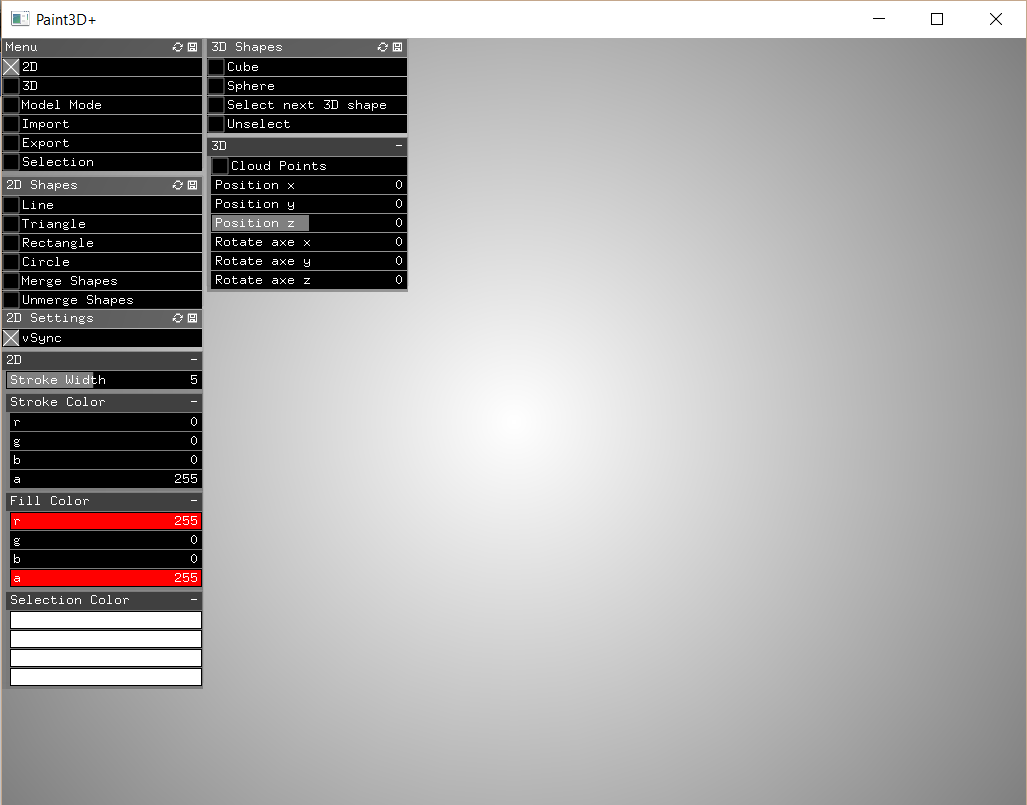
\includegraphics[scale=0.7]{fig/GUI_opening.png}
	\caption{Interface graphique � l'ouverture}
 \label{fig:f_gui}
\end{figure}

Voici un aper�u de l'interface graphique lors de l'ajout de formes 2D.

\begin{figure}[hb]
 \centering
 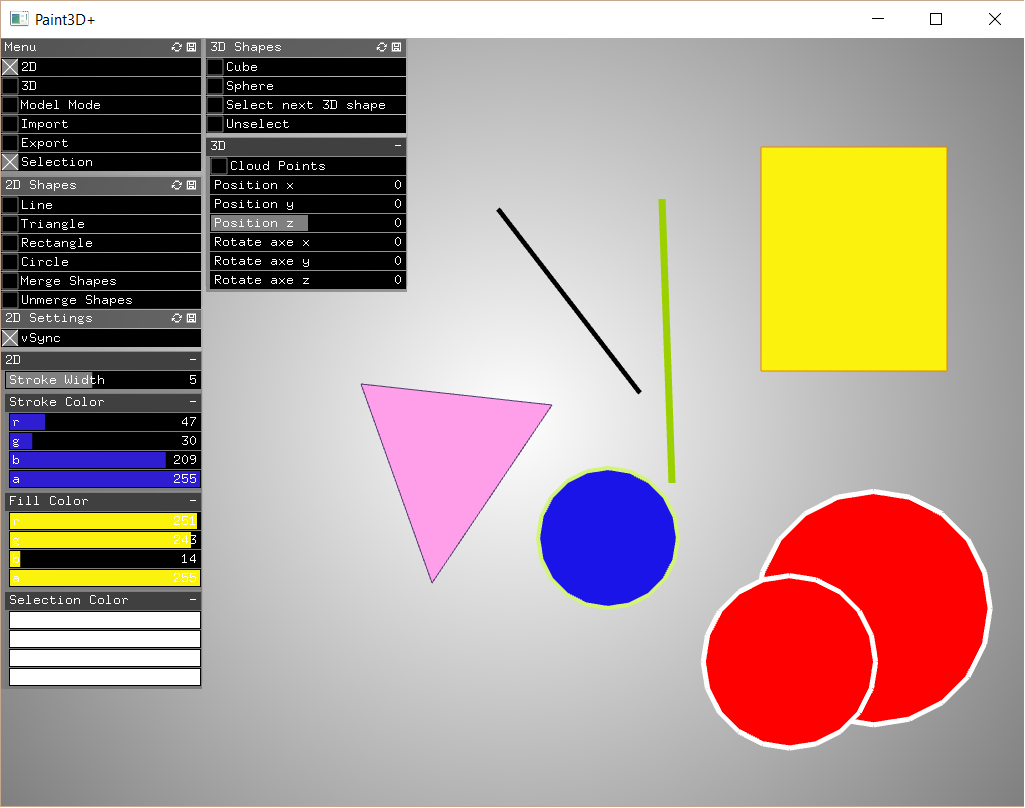
\includegraphics[scale=0.7]{fig/GUI_shapes2D.png}
	\caption{Interface graphique en mode 2D}
 \label{fig:f_gui2d}
\end{figure}

\begin{figure}[hb]
 \centering
 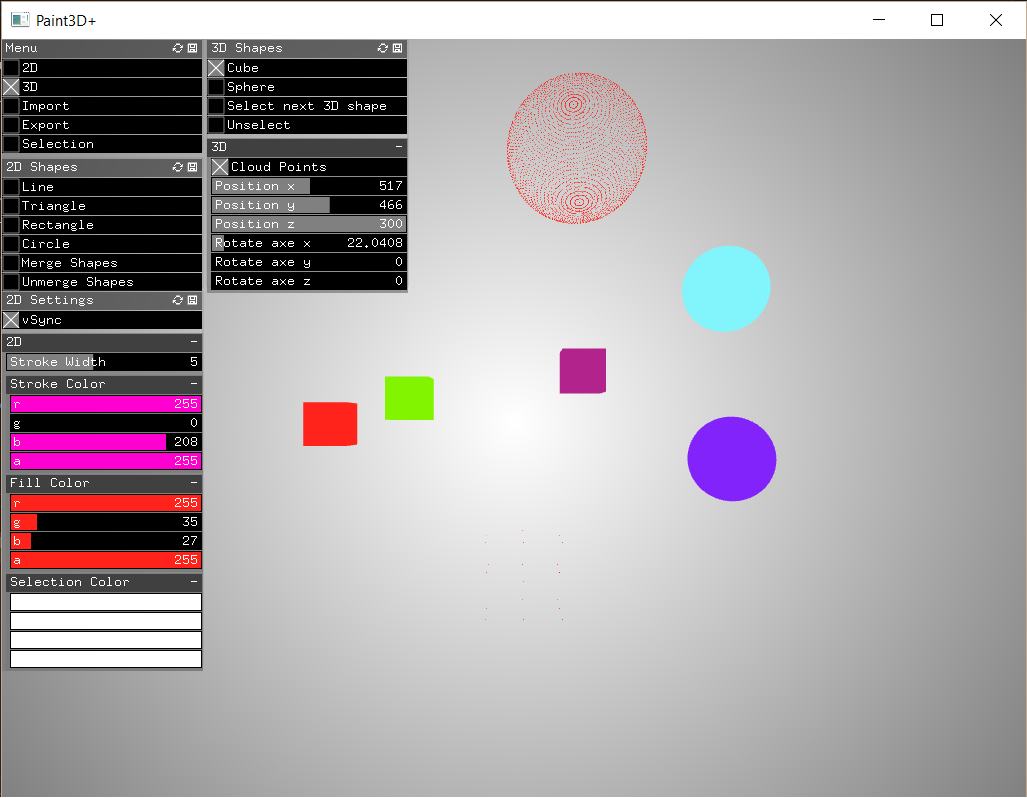
\includegraphics[scale=0.7]{fig/GUI_shape3D.png}
	\caption{Interface graphique en mode 3D}
 \label{fig:f_gui3d}
\end{figure}

\begin{figure}[hb]
 \centering
 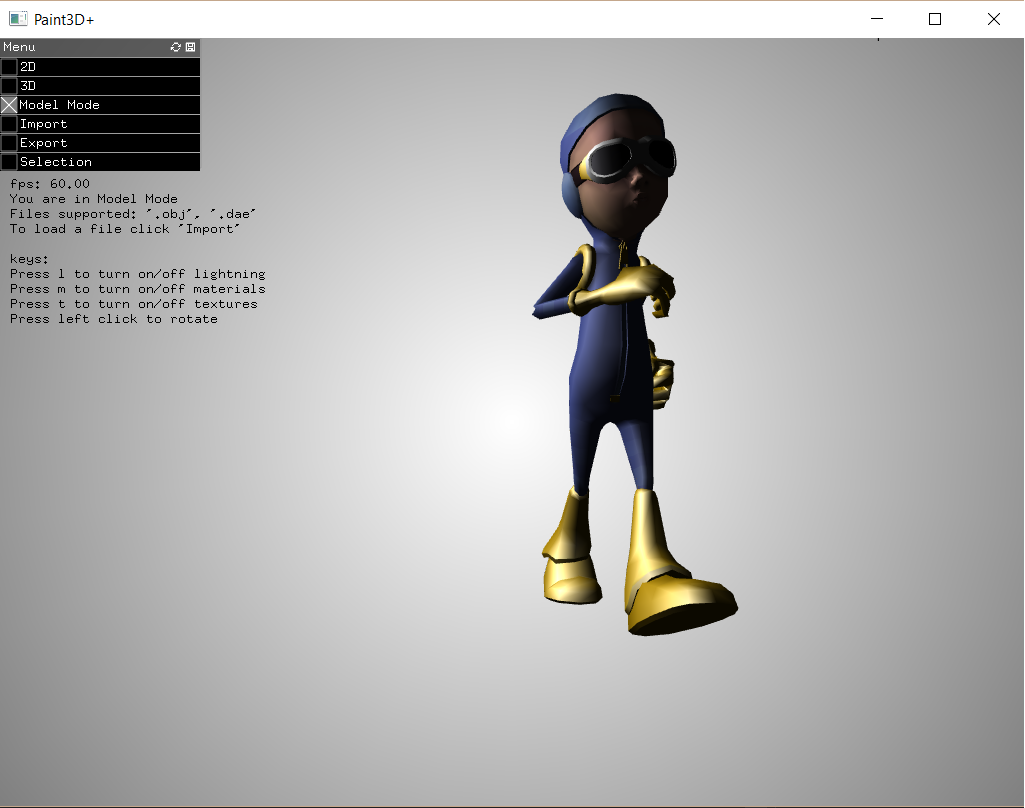
\includegraphics[scale=0.7]{fig/GUI_model.png}
	\caption{Interface graphique en mode mod�le}
 \label{fig:f_guiModel}
\end{figure}

\section{D�tails de l'interface graphique}
L'interface graphique permet de choisir une sc�ne de rendu 2D, 3D ou de mod�le selon le choix de l'utilisateur. De plus, il est possible d'importer des images en mode 2D et d'exporter la sc�ne sous forme d'image de format png � l'aide d'un dialogue de d'importation ou d'exporation. Le dernier item de la section Menu permet la s�lection des diff�rents objets de la sc�ne 2D.

\bigskip
\begin{itemize}
\item \textbf{2D} : Permet l'�dition d'une sc�ne de rendu 2D.
\item \textbf{3D} : Permet l'�dition d'une sc�ne de rendu 3D.
\item \textbf{Model Mode} : Permet l'importation d'un mod�le 3D.
\item \textbf{Import} : Permet l'importation d'une image dans la sc�ne.
\item \textbf{Export} : Permet l'expotation de la sc�ne de rendu, sans les diff�rents menus, sous forme d'une image de format png.
\item \textbf{Selection} : Permet la s�lection d'un ou de plusieurs objets 2D.
\end{itemize}

\subsection{2D Shapes}

Il est possible de dessiner quatre sortes de primitives vectorielles, en plus d'offrir la possibilit� de fusioner ces primitives, une fois qu'elles sont cr��es, ou de les d�fusioner avec les boutons Merge Shapes et Unmerge Shapes.

Dans le cas de la ligne, du rectangle et du cercle, l'utilisateur clique en un premier point et se d�place dans l'�cran afin de cliquer une seconde fois et former la primitive.

Pour ce qui est du triangle, l'utilisateur doit cliquer en trois points diff�rents.

\bigskip
\begin{itemize}
\item \textbf{Line} : Permet la cr�ation d'une ligne.
\item \textbf{Triangle} : Permet la cr�ation d'un triangle.
\item \textbf{Rectangle} : Permet la cr�ation d'un rectangle.
\item \textbf{Circle} : Permet la cr�ation d'un cercle.
\item \textbf{Merge Shapes} : Permet la cr�ation d'un objet 2D regroupant les formes s�lection�es.
\item \textbf{Unmerge Shapes} : Permet de d�truire l'objet 2D issu d'une fusion de formes. Les primitives vectorielles peuvent donc �tre manipul�es individuellement.
\end{itemize}

\subsection{2D}

Cette section de l'interface graphique regroupe les options de lignes de contour et de remplissage.

\bigskip
\begin{itemize}
\item \textbf{Stroke Width} : Permet l'ajustement de la largeur de la ligne de contour entre 1 et 10.
\item \textbf{Stroke Color} : Permet l'ajustement de la couleur de la ligne de contour sous forme RGBA.
\item \textbf{Fill Color} : Permet l'ajustement de la couleur de remplissage sous forme RGBA.
\item \textbf{Selection Color} : Permet l'ajustement de la couleur de s�lection sous forme RGBA. Cette couleur permet de d�terminer quel ou quels objets 2D sont s�lectionn�s en modifiant la couleur de la ligne de contour lors d'une s�lection.
\end{itemize}

\subsection{3D Shapes}

Cette section de l'interface graphique permet de faire l'ajout de formes 3D lorsque le mode 3D est activ�.

\bigskip
\begin{itemize}
\item \textbf{Cube} : Permet d'ajouter un cube.
\item \textbf{Sphere} : Permet d'ajouter une sph�re.
\item \textbf{Select next 3D shape} : Permet de parcourir et s�lectionner les formes 3D une � une.
\item \textbf{Unselect} : Permet de d�s�lectionner une objet 3D.
\end{itemize}

\subsection{3D}

Cette section de l'interface graphique permet de faire l'ajout de formes 3D lorsque le mode 3D est activ�.

\bigskip
\begin{itemize}
\item \textbf{Cloud points} : Permet d'ajouter un cube.
\item \textbf{Position x/y/z} : Permet de changer la position de l'objet 3D selon l'axe d�sir�.
\item \textbf{Rotate x/y/z} : Permet d'effectuer une rotation de l'objet 3D autour de l'axe d�sir�.
\end{itemize}

\section{Utilisation de la souris et racourcis clavier}

Lorsque l'utilisateur s�lectionne l'une ou l'autre des primitives verctorielles, le curseur change de forme afin de permettre � ce dernier de visualiser dans quel mode il se situe. Pour la s�lection il s'agit d'un curseur normal, tandis que pour les diff�rentes formes, le curseur prend l'apparence de la forme s�lectionn�e. Lorsque la souris se retrouve au dessus des diff�rents panneaux de configuration le curseur reprend sa forme normale.

Voici les diff�rentes fonctions de la souris selon les modes.

\subsection{2D}

\begin{itemize}
\item \textbf{Clic gauche} : Permet la s�lection d'un objet 2D.
\item \textbf{Clic gauche et d�placement} : Permet la s�lection d'objets dont au moins un coin touche � la zone de s�lection trac�e.
\item \textbf{Clic droit et ctrl} : Permet la s�lection multiple.
\item \textbf{Clic droit et d�placement} : Permet le d�placement d'un ou de plusieurs objet 2D.
\item \textbf{Clic droit et gauche} : Permet la rotation d'un ou de plusieurs objets 2D.
\item \textbf{Clic gauche et d�placement} : Permet d'ajuster la taille d'un ou de plusieurs objets 2D.
\item \textbf{Touche supprimer} : Permet de supprimer un objet 2D.
\end{itemize}


\subsection{3D}

\begin{itemize}
\item \textbf{Touche supprimer} : Permet la suppression de l'objet s�lectionn�.
\end{itemize}

\subsection{Model Mode}

Lorsqu'on entre en mode mod�le l'interface graphique change quelque peu afin d'afficher les raccourcis clavier � l'�cran.

\begin{itemize}
\item \textbf{Clic gauche et d�placement} : Permet une rotation du mod�le.
\item \textbf{Touche l} : Permet d'appliquer ou non une lumi�re.
\item \textbf{Touche m} : Permet d'appliquer ou non un mat�riau.
\item \textbf{Touche t} : Permet d'appliquer ou non une texture.
\end{itemize}
%!TEX encoding = IsoLatin

%
% Chapitre "Fonctionnalites"
%

\chapter{Technologie}

Voici les principaux outils utilis�s pour la r�alisation du projet.

Tout d'abord, OpenFrameworks est utilis� en tant que framework de programmation graphique. Pour ce qui est de l'environnement de d�veloppement, Visual Studio est celui employ�. 

%!TEX encoding = IsoLatin

%
% Chapitre "Architecture"
%

\chapter{Architecture}

Paint3D+ est organis�e en plusieurs classes qui supportent ces fonctionnalit�s. La structure 
hi�rarchique permet de minimaliser le volume du code n�cessaire et de faciliter l'impl�mentation de plusieurs fonctions (comme les transformations interactives, la s�lection multiple, etc.). Comme le programme fonctionne en 3 mods diff�rents, on peut grouper les classes en 3 parties respectivement: les classes qui supportent le mode 2D, le mode 3D et la partie du rendu qui est construite autour de la casse ''OfApp'' (fournie initialement par Openframworks).
\\

La vue d'ensemble est repr�sent�e dans la figure suivante:

\begin{figure}[h] 
\begin{center}
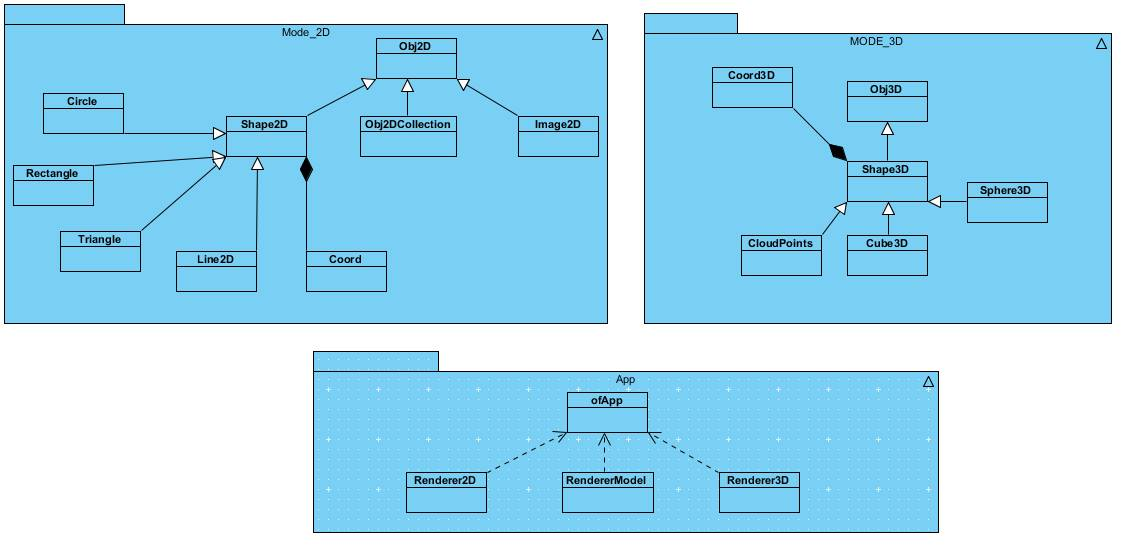
\includegraphics[width=15cm, height=10cm]{fig/uml1.jpg}
\end{center}
\caption{Diagramme UML vue d'ensemble.}
\end{figure}

Les d�tails pertinents de chaque classe sont pr�sents dans les diagrammes suivants:

\newpage

\begin{figure}[h] 
\begin{center}
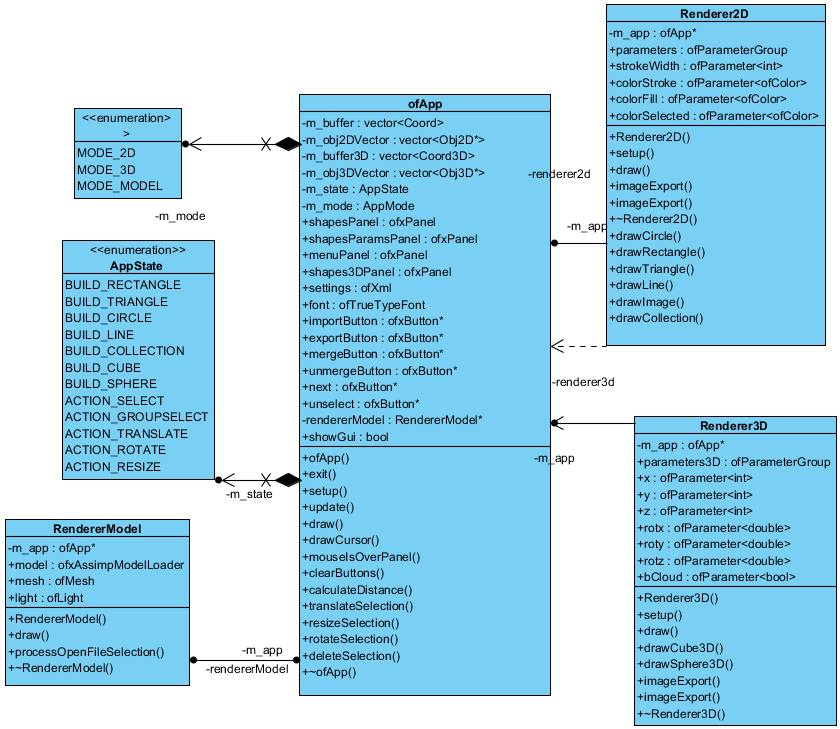
\includegraphics[width=15cm, height=10cm]{fig/uml2.jpg}
\end{center}
\caption{Diagramme UML de ofApp.}
\end{figure}

\begin{figure}[h] 
\begin{center}
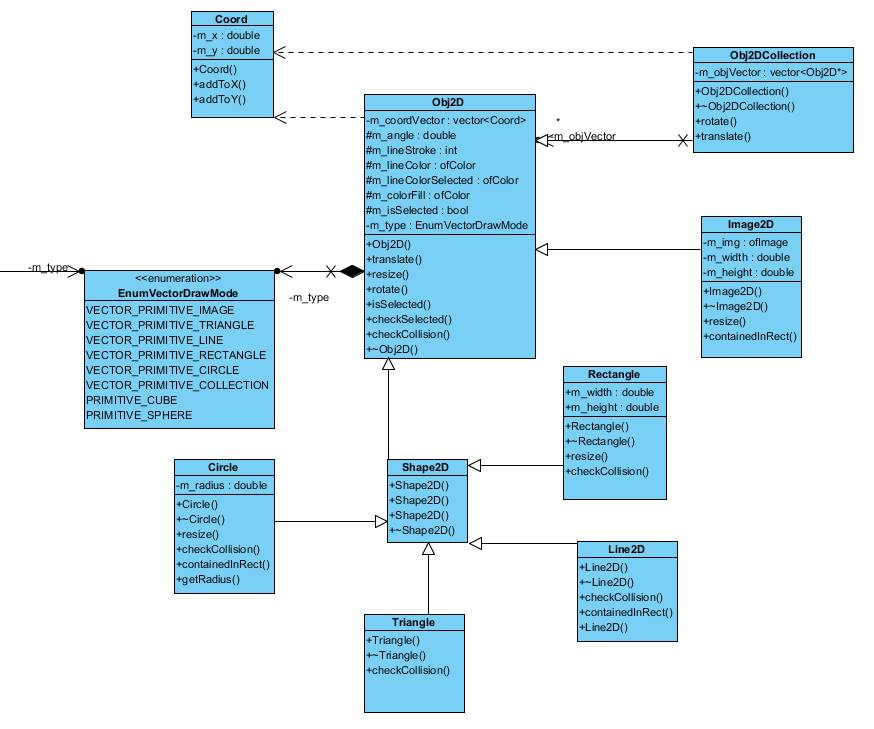
\includegraphics[width=15cm, height=10cm]{fig/uml3.jpg}
\end{center}
\caption{Diagramme UML du 2D.}
\end{figure}

\begin{figure}[h] 
\begin{center}
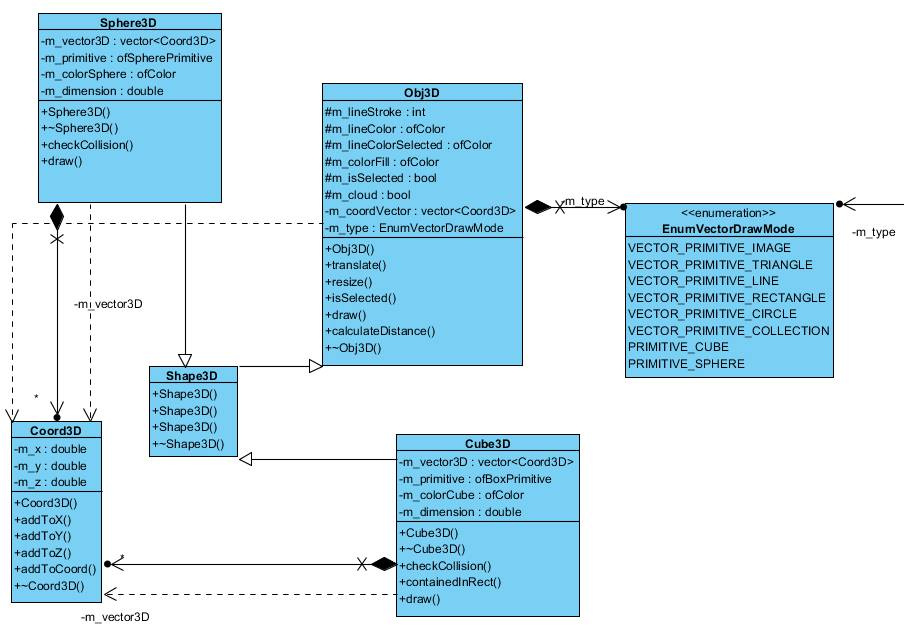
\includegraphics[width=15cm, height=10cm]{fig/uml4.jpg}
\end{center}
\caption{Diagramme UML du 3D.}
\end{figure}

\newpage 

Il faut tenir compte que le r�le de ces diagrammes est de montrer l'architecteur de l'application et la logique de fonctionnement (par exemple les m�thodes ''set'' et "get')' ont �t� omises pour simplifier la complexit� des diagrammes. Pour plus de d�tails, il faut consulter leur impl�mentation (le code dans les fichier .h et .cpp respectivement).
%!TEX encoding = IsoLatin

%
% Chapitre "Fonctionnalites"
%

\chapter{Fonctionnalit�s}

\section{Image}

\section{Dessin vectoriel}

\section{Transformation}



\section{G�om�trie}



\subsection{Particules}

Pour respecter ce crit�re fonctionnel, l'application doit rendre un nuage de points en une seule commande d'affichage.

Dans l'application Paint3D+,  il y a un bouton nomm� ''Cloud Points'' qui permet de transformer un objet 3D s�lectionn� en  un nuage de points o� chaque point est un sommet d'unedes faces qui compose l'objet en 3D.

Donc, pour pouvoir utiliser cette option, il faut cr�er un objet 3D avec le bouton ''Cube'' ou ''Sphere'' en mode 3D, s�lectionner un des objets 3D cr�� avec le bouton ''Select next 3D Shape'' et appuyer sur le bouton ''Cloud Points'' pour rendre l'objet 3D s�lectionn� en tant que nuage de points.

Les 2 figures suivantes montrent une sph�re rendue sans nuage de points et une sph�re rendue avec un nuage de points.

\begin{figure}[h] 
\begin{center}
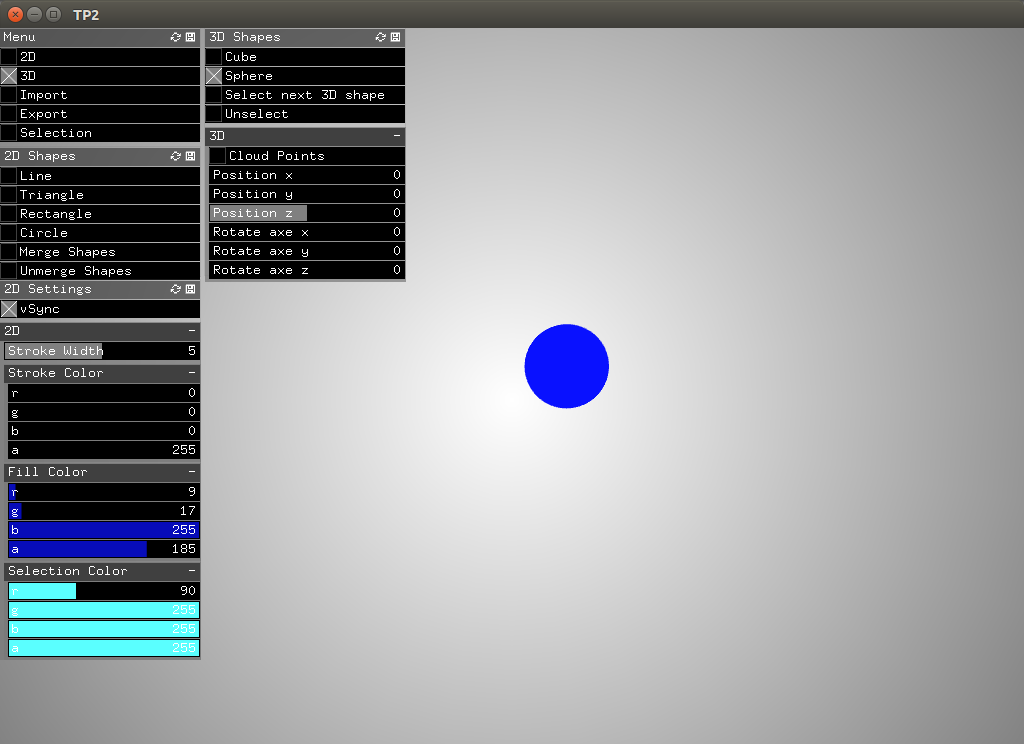
\includegraphics[width=13cm, height=13cm]{fig/cloudpoints1.png}
\end{center}
\caption{Une sph�re rendue sans nuage de points.}
\end{figure}
 
 
\begin{figure}[h] 
\begin{center}
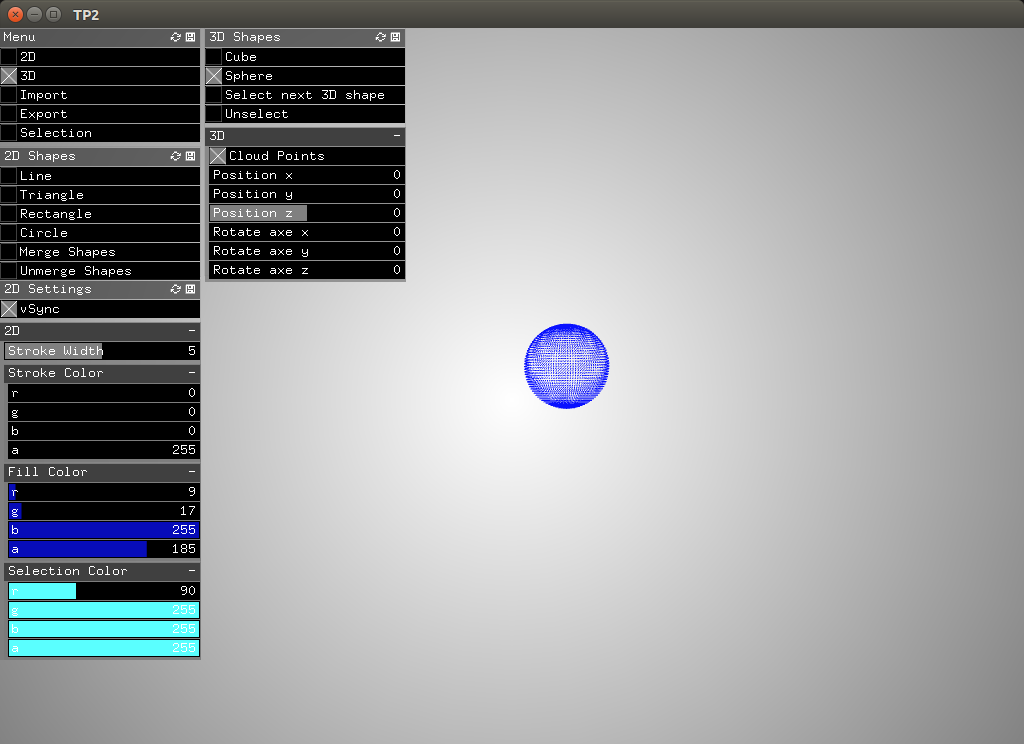
\includegraphics[width=13cm, height=13cm]{fig/cloudpoints2.png}
\end{center}
\caption{Une sph�re rendue avec un nuage de points.}
\end{figure}

\newpage

\subsection{Primitives 3D}

L'application doit permettre de cr�er au moins 2 types de primitives g�om�triques 3D � partir d'un algorithme sans aucune donn�es externes � l'application.

L'application Paint3D+ permet de cr�er 2 primitives 3D localement sans donn�es externes, soit le cube et la sph�re. Ces 2 primitives 3D sont cr��es par composition � partir de 2 classes d'OpenFrameworks, soit OfSpherePrimitive et OfxBoxPrimitive. 

Pour cr�er ces 2 primitives 3D, il faut d'abord s�lectionner le mode 3D dans le menu. Ensuite, il faut cocher soit Cube ou Sphere, selon la primitive 3D � cr�er et cliquer gauche sur la souris � l'endroit o� l'on veut que la primitive 3D apparaisse. Ensuite, pour modifier une primitive 3D cr��e, il faut la s�lectionner avec l'option ''Select next 3D shape'' et modifier les param�tres modifiables, soit la position en x,y,z l'orientation en x,y,z ou la couleur de s�lection ou de remplissage. 

Il est � noter que la rotation est faite � partir de quaternions dans le code.


\section{Illumination}

gggg
gggg
gggg
gg
%!TEX encoding = IsoLatin

%
% Chapitre "Ressources"
%

\chapter{Ressources}
Comme notre application repr�sente un outil de dessin, on n'a pas utilis� beaucoup de ressources externes (des diff�rentes images, shaders, etc.). Les ressources utilis�es pour accomplir le travail sont les ''addons'' et la documentation officielle de ''Openframeworks'' (http://openframeworks.cc/documentation/). Pour construire l'interface graphique,on a utilis� le module ''ofxGui''. Cela nous a permis d'ajouter les diff�rents boutons, le menu et les composantes pour modifier les param�tres des primitives dessin�es. Pour lire et rendre les fichiers mod�les, on a utilis� le module ''ofxAssimpModelLoader'' (inclus en openframeworks aussi). La librairie ''OpenGl'' a �t� utilis�e surtout pour repr�senter l'ombre sur les mod�les (GL\_SMOOTH shading). Pour manipuler les entit�s 3D, on utilise ''ofxOpenCv''. 
\\

On a utilis� �galement les librairies standard de C++ (<cmath>, <vector>) pour faire les op�rations math�matiques et pour utiliser des structures de donn�es qui contiennent des r�f�rences vers les objets instanci�s.
%!TEX encoding = IsoLatin

%
% Chapitre "Pr�sentation"
%

\chapter{Pr�sentation}

L'�quipe de d�veloppement est compos� de 4 membres qui ont travaill� dans une symbiose fructueuse. Cela a permis d'effectuer un travail conforme aux exigences du cours. Plusieurs moyens de communication ont �t� utilis�s pour l'organisation de travail et la r�partition des t�ches. Pour la planification de travail, nous avons prioris� les rencontres en personnes tandis que la phase de construction de l'application a �t� r�alis�e surtout � l'aide des rencontres virtuelles (skype). �galement, la plateforme ''Github'' a �t� un outil indispensable pour le partae du code et la fusion des parties. � part le c�t� technique, la collaboration de tos les membres de l'�quipe a �t� essentielle. On a essay� d'int�grer le plus souvent les fonctionnalit�s et GitHub a �t� indispenpensable pour accomplir cela. De cette fa�on, on a r�duit le risque de conflits et on a d�tect� le plus vite possible les erreurs de d�veloppement (qui surviennent dans le cycle de vie du processus). L'int�gration continue implique de faire de petits changements au logiciel en lui appliquant des tests de qualit� (si les erreurs sont d�tect�es plus tard dans le processus de d�veloppement, leurs corrections sont plus difficiles).
\\

\noindent Les membres de l'�quipe et leur programme d'�tude:
\\

\noindent Gabriel Lefran�ois: g�nie informatique\\
Marcel Bernic: baccalaur�at en informatique\\
Martin Richard Cerda: g�nie informatique\\
William-Jos� Simard-Touzet: g�nie informatique


%%!TEX encoding = IsoLatin

%
% Chapitre "Bibliographie"
%

\begin{thebibliographyUL}{99} % remplacer le "{9}" par "{99}" lorsque le nombre de references
                              % requiert 2 caracteres (>= 10 references)
                              
\bibitem{alimentationport} Conrad \textit{Blocs d'alimentation adapt�s pour PC portable}, [En ligne]. \url{http://www.conrad.fr/ce/fr/content/ti_NotebookNetzteile/Das-passende-Netzteil-fuer-Ihr-Netbook-bzw-Notebook-Conrad} (Page consult�e le 11 avril 2015) 

\bibitem{distQcMtl} Transports Qu�bec \textit{Outil d'estimation des distances routi�res } , [En ligne]. \url{http://www.quebec511.info/fr/distances/index1.asp} (Page consult�e le 08 avril 2015)                              
                              
\bibitem{Falgo} Wikipedia \textit{Fr�quence d'�clairage imperceptible} , [En ligne].\url{http://en.wikipedia.org/wiki/Flicker_(screen)} (Page consult�e le 06 avril 2015)

\bibitem{CapSE} TRI-TRONICS. \textit{SMARTEYE� COLORWISE�} , [En ligne]. \url{http://www.ttco.com/industrial/colorwise.aspx} (Page consult�e le 14 mars 2015)

\bibitem{prixCapSE} TRI-TRONICS. \textit{COLORWISE Products} , [En ligne]. \url{http://www.ttco.com/store/ItemList_Abstract.aspx?Category=COLORWISE+Products} (Page consult�e le 26 mars 2015)

\bibitem{CapTAOS} TAOS. \textit{TCS230 PROGRAMMABLE COLOR LIGHT-TO-FREQUENCY CONVERTER}, [En ligne]. \url{http://www.pobot.org/IMG/pdf/tcs230_datasheet.pdf} (Page consult�e le 14 mars 2015)

\bibitem{prixCapTAOS} Smart Prototyping. \textit{GY-31 TCS230 TCS3200 Color Sensor Recognition}, [En ligne]. \url{http://smart-prototyping.com/GY-31-TCS230-TCS3200-Color-Sensor-Recognition-Module-for-Arduino.html} (Page consult�e le 26 mars 2015)


\bibitem{CapHDJD} AVAGO TECHNOLOGIE. \textit{HDJD-S822-QR999 RGB Color Sensor}, [En ligne]. \url{http://dlnmh9ip6v2uc.cloudfront.net/datasheets/Sensors/LightImaging/HDJD-S822-QR999.pdf} (Page consult�e le 14 mars 2015)

\bibitem{prixCapHDJD} SparkFun. \textit{Color Sensor Breakout - HDJD-S822}, [En ligne]. \url{https://www.sparkfun.com/products/10904} (Page consult�e le 26 mars 2015)


\bibitem{Rout1} AMAZON. \textit{D-Link DI-514 Wireless Cable/DSL Router}, [En ligne]. \url{http://www.amazon.com/D-Link-DI-514-Wireless-Router-802-11b/dp/B000088NO8} (Page consult�e le 15 mars 2015)

\bibitem{Rout2} \textit{Wi-Fi}, [En ligne].\url{http://fr.wikipedia.org/wiki/Wi-Fi} (Page consult�e le 15 mars 2015)

\bibitem{blue1} rp electronics. \textit{OSEPP� Bluetooth}, [En ligne]. \url{https://www.rpelectronics.com/osepp-bth-01-arduino-compatible-microcontroller-bluetooth.html} (Page consult�e le 15 mars 2015)

\bibitem{blue2} \textit{Bluetooth}, [En ligne]. \url{http://fr.wikipedia.org/wiki/Bluetooth} (Page consult�e le 15 mars 2015)

\bibitem{sitecour} Lamontagne, Luc. \textit{Technique 3 � Quelques �l�ments de conception logicielle}, [En ligne]. \url{http://wcours.gel.ulaval.ca/2015/h/GEL1001/default/5chronologie/conception_logicielle.pdf} (Page consult�e le 15 mars 2015)

\bibitem{1dig} Digi-Key. \textit{Lite-On Inc LSHD-5601}, [En ligne]. \url{http://www.digikey.ca/product-detail/en/LSHD-5601/160-1575-5-ND/560008} (Page consult�e le 15 mars 2015)

\bibitem{4dig} Digi-Key. \textit{Lite-On Inc LTC-4727JR}, [En ligne]. \url{http://www.digikey.ca/product-detail/en/LTC-4727JR/160-1551-5-ND/408224} (Page consult�e le 15 mars 2015)

\bibitem{1bout} Conrad. \textit{Bouton Jtp-1230A Namae Electronics JTP-1130A}, [En ligne]. \url{http://www.conrad.fr/ce/fr/product/705260/Bouton-Jtp-1230A-Namae-Electronics-JTP-1130A;jsessionid=479A08C48C6FD4E768449D427E38E54A.ASTPCEN31?ref=list} (Page consult�e le 16 mars 2015) 

\bibitem{plaqV} Digi-Key. \textit{Hammond Manufacturing 1593LPCB}, [En ligne]. \url{http://www.digikey.ca/product-detail/en/1593LPCB/HM1253-ND/2359724} (Page consult�e le 16 mars 2015)

\bibitem{EcrSS} Sain Smart. \textit{SainSmart 3.2" SSD1289 Touch Screen With MicroSD For Arduino Raspberry Pi}, [En ligne]. \url{http://www.sainsmart.com/sainsmart-3-2-tft-lcd-display-touch-panel-pcb-adapter-sd-slot-for-arduino-2560.html} (Page consult�e le 15 mars 2015)

\bibitem{BlindTac} RobotShop. \textit{Blindage LCD Tactile 2.8" pour pcDuino/Arduino}, [En ligne]. \url{http://www.robotshop.com/ca/fr/blindage-lcd-tactile-28-pcduino-arduino.html} (Page consult�e le 14 mars 2015)

\bibitem{BlindBout} RobotShop. \textit{Blindage LCD + Boutons pour Arduino DFRobot}, [En ligne]. \url{http://www.robotshop.com/ca/fr/blindage-lcd-boutons-arduino-dfrobot.html} (Page consult�e le 14 mars 2015)

\bibitem{HughesPrice} Hughes. \textit{Hughes 9202 BGAN Satellite Terminal}, [En ligne]. \url{http://www.groundcontrol.com/Hughes_9202_BGAN.htm} (Page consult�e le 19 mars 2015)

\bibitem{Rogers} Rogers. \textit{La LTE de Rogers}, [En ligne]. \url{www.rogers.com/lalte/} (Page consult�e le 19 mars 2015)

\bibitem{Xplornet} Xplornet. \textit{Plans and pricing}, [En ligne]. \url{http://www.xplornet.com/plans-pricing/residential-plans-pricing/} (Page consult�e le 19 mars 2015)

\bibitem{SamsungPrix} ebay. \textit{Samsung Galaxy Note 4 N910H}, [En ligne]. \url{http://www.ebay.com/itm/New-Samsung-Galaxy-Note-4-N910H-32GB-Factory-Unlocked-GSM-Phone-all-colors-/351310585533} (Page consult�e le 9 avril 2015)

\bibitem{LenoC40} Apple store. \textit{Lenovo C40}, [En ligne]. \url{http://www.futureshop.ca/fr-CA/product/lenovo-ordinateur-tout-en-un-21-5-po-c40-lenovo-a6-6310-amd-dd-1-to-ram-8-go-radeon-r4-amd-windows-8-1-f0b5002kcf/10360968.aspx?path=d657c0634bb8cc6e67fa928123d2e410fr02} (Page consult�e le 27 mars 2015)

\bibitem{Lenovo} Lenovo. \textit{ThinkPad X250}, [En ligne]. \url{http://shop.lenovo.com/us/en/laptops/thinkpad/x-series/x250/} (Page consult�e le 19 mars 2015)

\bibitem{BGAN} Immarsat. \textit{E-SAT}, [En ligne]. \url{http://www.e-sat.fr/fr/reseaux/inmarsat-bgan/#.VQtf7FxTMpw} (Page consult�e le 19 mars 2015)

\bibitem{lumenbeam} lumenpulse. \textit{Lumenbeam Small Color Changing}, [En ligne]. \url{http://www.lumenpulse.com/fr/produit/25/lumenbeam-small-color-changing}, (Page consult�e le 16 mars 2015).

\bibitem{lumenbeamprice} Farralane. \textit{Color Kinetics ColorBurst Compact Powercore}, [En ligne]. \url{http://www.farralane.com/store/p-5374-color-kinetics-colorburst-compact-powercore.aspx}, (Page consult�e le 19 mars 2015).

\bibitem{molveno} Molveno, \textit{RBG LED Systems}, [En ligne]. \url{http://www.molvenolighting.com/led/6RGBLedSystemsbassa-opt.pdf} (Page consult�e le 19 mars 2015).

\bibitem{molvenoprice}EMCOM, \textit{Catalogue g�n�ral 3}, [En ligne]. \url{http://www.emcom.ch/cat-interactifs/G3/files/assets/basic-html/page67.html}  (Page consult�e le 19 mars 2015).

\bibitem{supportmolveno} Espaceampouleled, \textit{Encastrable led orientable Spot escargot rond, 30W, blanc neutre }, [En ligne] \url{http://www.leclubled.fr/spots-led-encastrables/202-spot-encastrable-orientable-rond-blanc-type-escargot-0615872254361.html#/couleur-blanc/douille-mr16} (Page consult�e le 13 avril 2015).

\bibitem{molvenoangle} Le club LED, \textit{Spot encastrable orientable rond blanc - type escargot}, [En ligne] \url{http://www.espaceampouleled.fr/spot-escargot-rond-30w-blanc-neutre,fr,4,7674.cfm} (Page consult�e le 13 avril 2015).

\bibitem{ruban} Superbrightleds,\textit{LED Light Strips with Multi Color LEDs}, [En ligne]. \url{https://www.superbrightleds.com/moreinfo/rgb-bars-and-strips/led-light-strips-with-multi-color-leds-led-tape-light-with-18-smdsft-3-chip-rgb-smd-led-5050-with-lc4-connector/1470/#/tab/Specifications} (Page consult�e le 19 mars 2015).


\bibitem{Com1} UMQ \textit{Enqu�te qu�b�coise sur l'acc�s des m�nages � Internet}, [En ligne]. \url{http://www.umq.qc.ca/nouvelles/actualite-municipale/enquete-quebecoise-sur-l-acces-des-menages-a-internet-08-10-2013} (Page consult�e le 17 mars 2015)

\bibitem{Com2} Tyseo Web \& Marketing \textit{Planning type de cr�ation web (PME, 20 pages)}, [En ligne]. \url{http://www.tyseo.net/temps-faire-site-internet.php} (Page consult�e le 17 mars 2015)

\bibitem{Com3} Emploi Qu�bec \textit{Programmeurs/programmeuses et d�veloppeurs/d�veloppeuses en m�dias interactifs (2174) Salaires et statistiques}, [En ligne] \url{http://imt.emploiquebec.gouv.qc.ca/mtg/inter/noncache/contenu/asp/mtg122_statprof_01.asp?PT4=53&lang=FRAN&Porte=1&cregncmp1=QC&cregncmp2=QC&cregn=QC&PT1=36&prov=pje&PT3=10&pro=2174&PT2=21} (Page consult�e le 17 mars 2015)

\bibitem{Com4} Clare-Marie Karat, Christine Halverson, Daniel Horn, and John Karat.  �Patterns of Entry and Correction in Large Vocabulary Continuous Speech Recognition Systems�. CHI 99 Conference Proceedings [En ligne].15-20 Mai 1999, p.571 \url{http://www-personal.umich.edu/~danhorn/reprints/horn_1999_speech_recognition_patterns_chi_99.pdf} (Page consult�e le 19 mars 2015)

\bibitem{Com5} metiers-quebec.org \textit{SALAIRE}, [En ligne] \url{http://www.metiers-quebec.org/communication/museologue.html} (Page consult�e le 17 mars 2015)

\bibitem{tablettec} ebay \textit{Tablette tactile 16go 10 pouces full hd 1080p capacitif wifi google play jeux}, [En ligne] \url{http://www.cafr.ebay.ca/itm/Tablette-tactile-16go-10-pouces-full-hd-1080p-capacitif-wifi-google-play-jeux-/141125695295?pt=LH_DefaultDomain_71&hash=item20dbbf373f} (Page consult�e le 9 avril 2015)






\bibitem{DD1} Linternaute. \textit{Disque dur ou service en ligne ?}, [En ligne]. \url{http://www.linternaute.com/photo_numerique/archivage/stocker-ses-photos-sans-risque/comment-choisir.shtml} (Page de consult�e le 18 mars) 

\bibitem{DD2} \textit{Disque dur}, [En ligne]. \url{http://fr.wikipedia.org/wiki/Disque_dur} (Page de consult�e le 18 mars) 

\bibitem{DDbestbuy} bestbuy.ca. \textit{
Disque dur interne de 2,5 po d'une capacit� de 1 To de Seagate (ST1000LM024) - En ligne seulement
}, [En ligne]. \url{http://www.bestbuy.ca/fr-CA/product/seagate-disque-dur-interne-de-2-5-po-d-une-capacite-de-1-to-de-seagate-st1000lm024-st1000lm024/10324346.aspx?path=fc95f447a9868023d87384981c7dd1bdfr02} (Page de consult�e le 10 avril 2015)


\bibitem{blueray1} Blu-Ray Disc. \textit{QU'EST-CE QUE LE BLU-RAY ?}, [En ligne]. \url{http://www.bluray-facile.com/} (Page de consult�e le 18 mars)

\bibitem{blueray2} \textit{Disque Blu-ray}, [En ligne]. \url{http://fr.wikipedia.org/wiki/Disque_Blu-ray} (Page de consult�e le 18 mars)

\bibitem{blueray3} Comment �a marche?.net. \textit{Explication d'un Blu ray disc?}, [En ligne]. \url{http://www.commentcamarche.net/forum/affich-7548383-explication-d-un-blu-ray-disc} (Page de consult�e le 18 mars)

\bibitem{blueray4} amazon.ca \textit{Verbatim Mitsubishi 50GB 2x Speed BD-RE Blu-ray Re-Writable Disk 5 Pack}, [En ligne]. \url{http://www.amazon.ca/Verbatim-Mitsubishi-Speed-Blu-ray-Re-Writable/dp/B004JKHRK8/ref=sr_1_fkmr1_2?ie=UTF8&qid=1428769246&sr=8-2-fkmr1&keywords=writable+blue+ray} (Page de consult�e le 9 avril 2015)

\bibitem{cloud1} iweb  \textit{Deploy a cloud server}, [En ligne]. \url{http://iweb.com/cloud/servers?pi_ad_id=50514088089&gclid=CNWUmdeH-cQCFQwzaQodIAIA0w} (Page de consult�e le 18 mars)


\bibitem{cleUSB1}  BestBuy.ca \textit{Cl� USB 3.0 de 32 Go JumpDrive de Lexar (LJDS33-32GASBNA) - Vert}, [En ligne]. \url{http://www.bestbuy.ca/fr-CA/product/lexar-media-cle-usb-3-0-de-32-go-jumpdrive-de-lexar-ljds33-32gasbna-vert-ljds33-32gasbna/10243190.aspx?path=0b1368b0b57d7f591cd5f32edce421c0fr02} (Page de consult�e le 10 avril)


\bibitem{cleUSB2}  \textit{Cl� USB}, [En ligne]. \url{http://fr.wikipedia.org/wiki/Cl\%C3\%A9_USB} (Page de consult�e le 10 avril)

\bibitem{Allen Bradley} ROCHWELL AUTOMATISATION. \textit{Syst�mes automates programmables MicroLogix 1200}, [En ligne]. \url{http://ab.rockwellautomation.com/fr/Programmable-Controllers/MicroLogix-1200\#overview} (Page de consult�e le 16 mars) 
\bibitem{Allen Bradley1} ALI EXPRESS. \textit{vente en gros allen bradley micrologix 1200}, [En ligne]. \url{http://fr.aliexpress.com/w/wholesale-allen-bradley-micrologix-1200.html} (Page consult�e le 16 mars)
\bibitem{Ismart V3} IMO. \textit{La solution ideal pour les constructeurs de machine}, [En ligne]. \url{http://www.imopc.com/content.php?p=spotlight_ismart&lang=FR} (Page consult�e le 16 mars)
\bibitem{Ismart V31} TECHNIC-ACHAT. \textit{automatisation et �lectricit� industrielle}, [En ligne]. \url{http://www.technic-achat.com/index.cfm} (Page consult�e le 16 mars)
\bibitem{Ismart V32} TECO. \textit{SG2 Smart PLC USER Manual}, [En ligne]. \url{http://www.bb-elec.com/Products/Manuals/SG2V3_UserManual.pdf} (Page consult�e le 12 avril)
\bibitem{berrypi} CANADA ROBOTIX. \textit{Rapsberry pi 2 model b 1GB}, [En ligne]. \url{http://www.canadarobotix.com/1426-raspberry-pi-2-model-b-1gb} (Page consult�e le 16 mars)
 
\bibitem{Rapsberry2} HELEN LYNN. \textit{RASPBERRY PI 2 MODEL B}, [En ligne]. \url{http://www.raspberrypi.org/products/raspberry-pi-2-model-b/} (Page consult�e le 16 mars)
\bibitem{Rapsberry3} MCM. \textit{Raspberry Pi� 2 Model B 1GB Project Board}, [En ligne].] \url{http://www.mcmelectronics.com/product/83-16530} (Page consut�e le 16 mars)
\bibitem{Arduino1} ARDUINO. \textit{what is Aduino}, [En ligne]. \url{http://arduino.cc/en/Main/ArduinoBoardMega2560} (Page consult�e le 16 mars)
\bibitem{Arduino2} ROBOSHOP. \textit{La boutique � votre service}, [En ligne]. \url{http://www.robotshop.com/ca/fr/microcontroleur-arduino-mega-2560-adk.html} (Page consult�e le 16 mars)



\end{thebibliographyUL}









\end{document}
% Fin du document

